% !TEX encoding = UTF-8 Unicode
\RequirePackage{fix-cm}
\documentclass[a4paper,10pt,UTF8]{paper}
%\documentclass[a4paper,10pt,UTF8]{ctexart}

\usepackage[english]{babel}
\usepackage{fancyhdr,array,lastpage,amsmath,mathtools,enumitem,graphicx,multirow,tocbibind,longtable,makecell,varwidth,titlesec,bm,booktabs,comment}
\usepackage{enumitem}
\usepackage{hyperref}
\hypersetup{hidelinks}
\usepackage{fontspec, xunicode, xltxtra}
\usepackage{xeCJK}%中文字体

% \setCJKmainfont{PingFang SC}
% \setmainfont{PingFang SC}
% \setCJKmonofont{PingFang SC}

\usepackage[left=2.54cm,right=2.54cm,top=2.54cm,bottom=2.54cm]{geometry}
\usepackage[font=footnotesize,labelfont=bf]{caption}
\usepackage{tikz,flowchart}
\usepackage{ctex}
\usetikzlibrary{shapes,shapes.geometric,arrows,matrix,calc}
\usetikzlibrary{circuits.logic}
% \usetikzlibrary{circuits.logic.custom}
\usetikzlibrary{circuits.logic.IEC}
\usetikzlibrary{shadows}
\usepackage{listings}
\usepackage[Q=yes]{examplep}
\usepackage{fancyhdr}
\usepackage{alphalph}
\usepackage{indentfirst}

\newenvironment{sol}
  {\par\vspace{2mm}\noindent{\bf Solution}. }

\lstset{escapeinside=``, breaklines=true, frame=none, extendedchars=false, basicstyle=\ttfamily, showstringspaces=false}


\setlength{\parindent}{2em}
\setlength{\parskip}{1.5ex plus 0.5ex minus 0.2ex}
\linespread{1.1}

\bibliographystyle{plain}

\numberwithin{equation}{section}
\numberwithin{figure}{section}

\usepackage{karnaugh}
\usepackage{circuitikz}


\setcounter{secnumdepth}{3}
\setcounter{tocdepth}{3}

\title{华东师范大学计算机科学技术系上机实验报告}

\begin{document}
\pagestyle{fancy}
\chead{\small\color{gray}华东师范大学计算机科学技术系上机实验报告}
\lhead{}
\rhead{}
\makeatletter
\def\headrule{{\if@fancyplain\let\headrulewidth\plainheadrulewidth\fi%
\color{gray}\hrule\@height 0.2pt\@width\headwidth}
  \vspace{6mm}}
\makeatother

\newcommand{\HRule}{\rule{\linewidth}{1mm}}
\newcommand{\dai}{\textbf{Dais-CMX16$^+$}}

{\center {\huge \bfseries \LARGE{华东师范大学计算机科学技术系上机实验报告}} \\ [0.8cm]

\small{
  \begin{minipage}[t]{.32\linewidth}
    \textbf{课程名称:}计算机组成与结构实践\\
    \textbf{指导教师:}金健\\
    \textbf{上机实践名称:} 存储器读写实验\\
    \textbf{实践编号:}实验 4
  \end{minipage}
  \begin{minipage}[t]{.32\linewidth}
    \textbf{年级:}17 级\\
    \textbf{姓名:}朱桐\\
    \textbf{学号:}10175102111\\
    \textbf{组号:}A
  \end{minipage} 
  \begin{minipage}[t]{.32\linewidth}
    \textbf{上机实践成绩:} \\
    \textbf{创新实践成绩:} \\
    \textbf{上机实践日期:}2019/10/11\\
    \textbf{上机实践时间:}2 学时\\
  \end{minipage}
}
\HRule \\[0.5cm]
}
\section{实验目的}

\begin{enumerate}
    \item 熟悉和了解存储器组织与总线组成的数据通路
\end{enumerate}

\section{实验设备}

\begin{enumerate}
    \item 指令寄存器,编译器
\end{enumerate}


\section{实验内容}
\subsection{实验连线}

\begin{figure}[h]
    \centering
    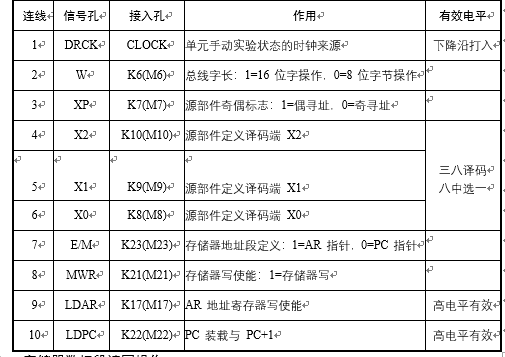
\includegraphics[width=0.8\linewidth]{1.PNG}
    \caption{实验连线}
    \label{fig:1}
\end{figure}

实验连线的图标如图 \ref{fig:1} 所示

\subsection{存储器数据段读写实验}

\subsubsection{数据段写操作}

在进行数据存储器字操作时,地址线 A0 必须为 0(偶地址)。向数据段的 0000~0005h 存储单元写入 11 22 33 44 55 66 一串数据,以 0000h 地址单元写入数据 1122h 为例表述操作流程。

\begin{itemize}
    \item $X_2X_1X_0=011, XP\ W=11,E/M=LDAR=1$ 按单拍,输入地址
    \item $LDAR=0$,输入数据 $1122$
    \item $MWR=1$,单拍,存储器写入
    \item $MWR=0$,关闭存储器写入
\end{itemize}

\subsubsection{数据段读入操作}

(2)	数据段读操作(字)依次读出数据段 0~0005h 单元的内容,这里以 0000h 地址单元读出为例阐述操作流程。

\begin{itemize}
    \item $X_2X_1X_0=011, XP\ W=11,E/M=LDAR=1$ 按单拍,输入地址
    \item $LDAR=0, X_2X_1X_0=100, W=1$ 存储器读入
\end{itemize}

执行上述流程总线单元应显示 1122h,若正确可按上述流程读出 0002~0005h 单元的内容。

\subsection{存储器程序段读写操作}

\subsubsection{程序段字节读写操作}

计算机规范的取指操作均以字节为单位,所以本实验以字节操作方式展开,程序段写入必须从定义地址入手,然后再进入程序存储器的写入。

PC 指针是带预置加法计数器,因此在输入起始地址后一旦后续地址为 PC+1 的话就不用重装 PC,用 PC+1 指令完成下续地址的读写操作。

PC 地址装在写入与 PC+1 写入流程:

\begin{itemize}
    \item 
\end{itemize}

\section{实验原理}

\section{实验步骤}

\section{调试过程、结果与分析}

\section{总结}

\section{附件}

\end{document}
